%% LyX 2.1.3 created this file.  For more info, see http://www.lyx.org/.
%% Do not edit unless you really know what you are doing.
\documentclass[english]{article}
\usepackage{ccfonts}
\usepackage[T1]{fontenc}
\usepackage[latin9]{inputenc}
\usepackage{geometry}
\geometry{verbose,tmargin=3cm,bmargin=3cm,lmargin=3cm,rmargin=3cm,headheight=3cm,headsep=3cm,footskip=3cm}
\usepackage{array}
\usepackage{url}
\usepackage{graphicx}
\usepackage{setspace}
\onehalfspacing

\makeatletter

%%%%%%%%%%%%%%%%%%%%%%%%%%%%%% LyX specific LaTeX commands.
%% Because html converters don't know tabularnewline
\providecommand{\tabularnewline}{\\}

%%%%%%%%%%%%%%%%%%%%%%%%%%%%%% User specified LaTeX commands.
\usepackage{listings}

\makeatother

\usepackage{babel}
\begin{document}

\title{Young's Modulus}


\author{Atul Singh Arora}


\date{March 2015}

\maketitle

\section{Theory}

The theory for this experiment has been primarily been adapted from
\url{http://www.animations.physics.unsw.edu.au//jw/elasticity.htm}.

Consider a typical wire. Stretching this leads to a small increase
in length of the wire. At the microscopic level, the average distance
between the atoms, $r$, increases. The attractive force between the
atoms balances slash resists the applied tensile force. 

Similarly, shortening a metal by applying a compressive force leads
to decrease in $r$ and is again balanced by inter-atomic repulsion.

From these one can deduce that 
\begin{itemize}
\item When $r>r_{eq}$ where $r_{eq}$ is the interatomic distance when
the wire is not under stress (will be defined precisely later), the
interatomic attraction is greater than repulsion.
\item When $r<r_{eq}$, the interatomic repulsion is greater than interatomic
attraction.
\end{itemize}
Further, from experience, we know that metals are harder to compress
which suggests
\begin{itemize}
\item Repulsive forces grow much more rapidly with $\left|r-r_{eq}\right|$
compared to the attractive force
\end{itemize}
And finally, we also know that once a metal is stretched beyond a
limit, it breaks and won't 'spring back together'. So we conclude
\begin{itemize}
\item If the interatomic distance $r>r_{max}$ (some $r_{max}$) then the
attractive forces become effectively zero.
\end{itemize}
Using these principels, we can plot the repulsive and attractive forces
as a function of $r$. We can also plot energy against $r$.

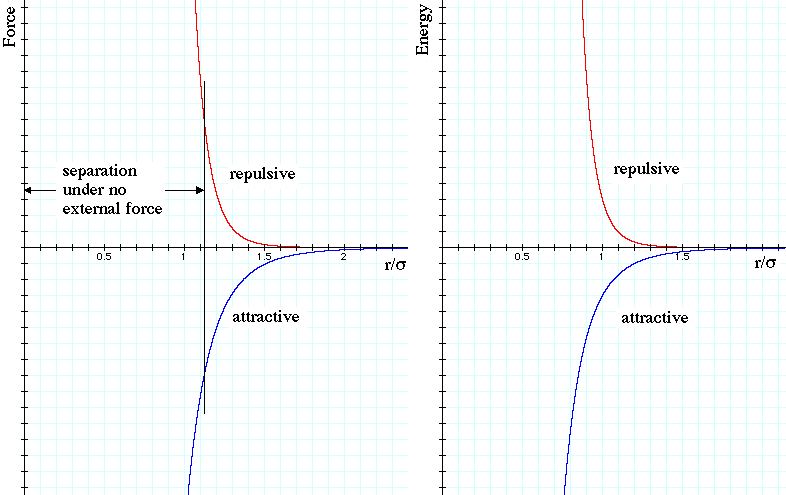
\includegraphics[width=16cm]{others/forcesalone}

We use the convention that repulsive forces are positive and attractive
are negative. Combining these graphs results in the following. One
must note that what we measure eventually is the combined effect of
the attractive and repulsive components. In this sense the division
between them is artificial. 

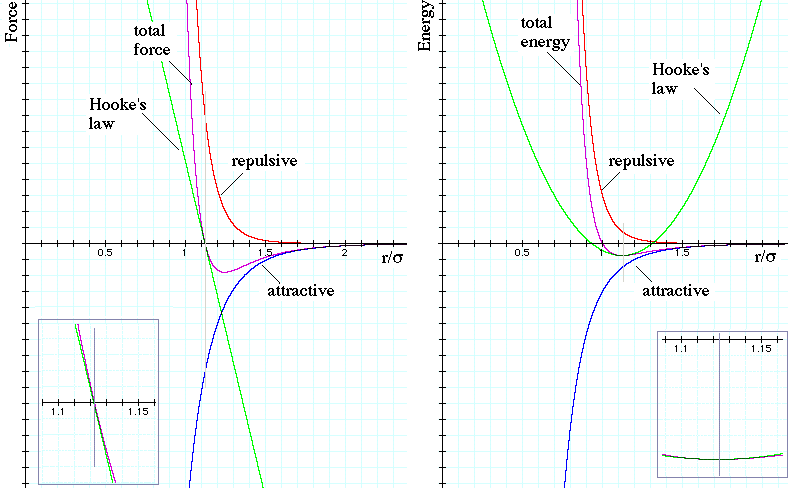
\includegraphics[width=16cm]{others/fitted}

Note that the Hook's law (yet to be stated explicitly) is valid in
the linear range of the force (and equivalently, the quadratic range
of the potential). This explains the microscopic origin of Hook's
law, which can be expressed in this context as
\[
F\propto-(r-r_{eq})
\]
Using this relation, one can write a more relavent quantity, the Young's
Modulus (which is defined such that it is fixed for a given material)
\[
Y=\frac{F/A}{\Delta l/l}
\]
where $F$ is the tensile force (for the wire say, that we considered
to start with), $A$ is the surface area normal to the force, $\Delta l$
is the change in length from the unstressed length (viz. when $F=0$),
and $l$ is the length when $F=0$.


\section{Experimental Setup}

The setup allows one to essentially stretch a wire with known weight,
as is required. Non-trivial aspects include a pulley (whose presence
is not included in the calculations) and a radial dial (1 division
= 0.25 cm) that measures $\Delta l$ with precision. The dial also
requires the wire to be looped around its knob two or three times.

The procedure is straight forward. One measures the length of the
wire (after making it taut preferably), fixes it on the setup so that
its taut. The wire is looped through the displacement dial and attached
to the weight through th pulley. Weight is added with as high a precision
as possible. Once the small weights are over (viz. all used), the
wire is removed and another wire is setup. This wire is now started
with the same old weight, except this time, low precision weights
are used to get the old weight. Subsequently, high precision weights
are added and the procedure continued till the wire breaks. Obviously,
the displacement is noted sensibly to account for consistency with
the previous sets of readings. This entire procedure is repeated with
a wire of a different material.


\section{Observations}


\subsection{Time-line}

\begin{tabular}{llp{9cm}}
\hline 
March 9 & Monday & Started performing the next experiment {[}didn't use mixed weights{]}\tabularnewline
March 10 & Tuesday & Performed the experiment for both Copper and Constantan using mixed
weights and multiple wires\tabularnewline
March 13 & Friday & Analyzed the data and worked on writing the record\tabularnewline
\hline 
\end{tabular}


\subsection{Constantan}

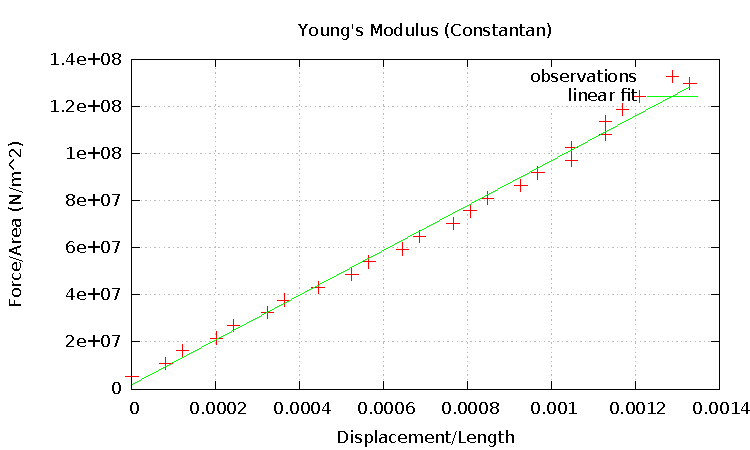
\includegraphics{exp5gnu/constantan}

\lstinputlisting{exp5gnu/constantanFit.tex}

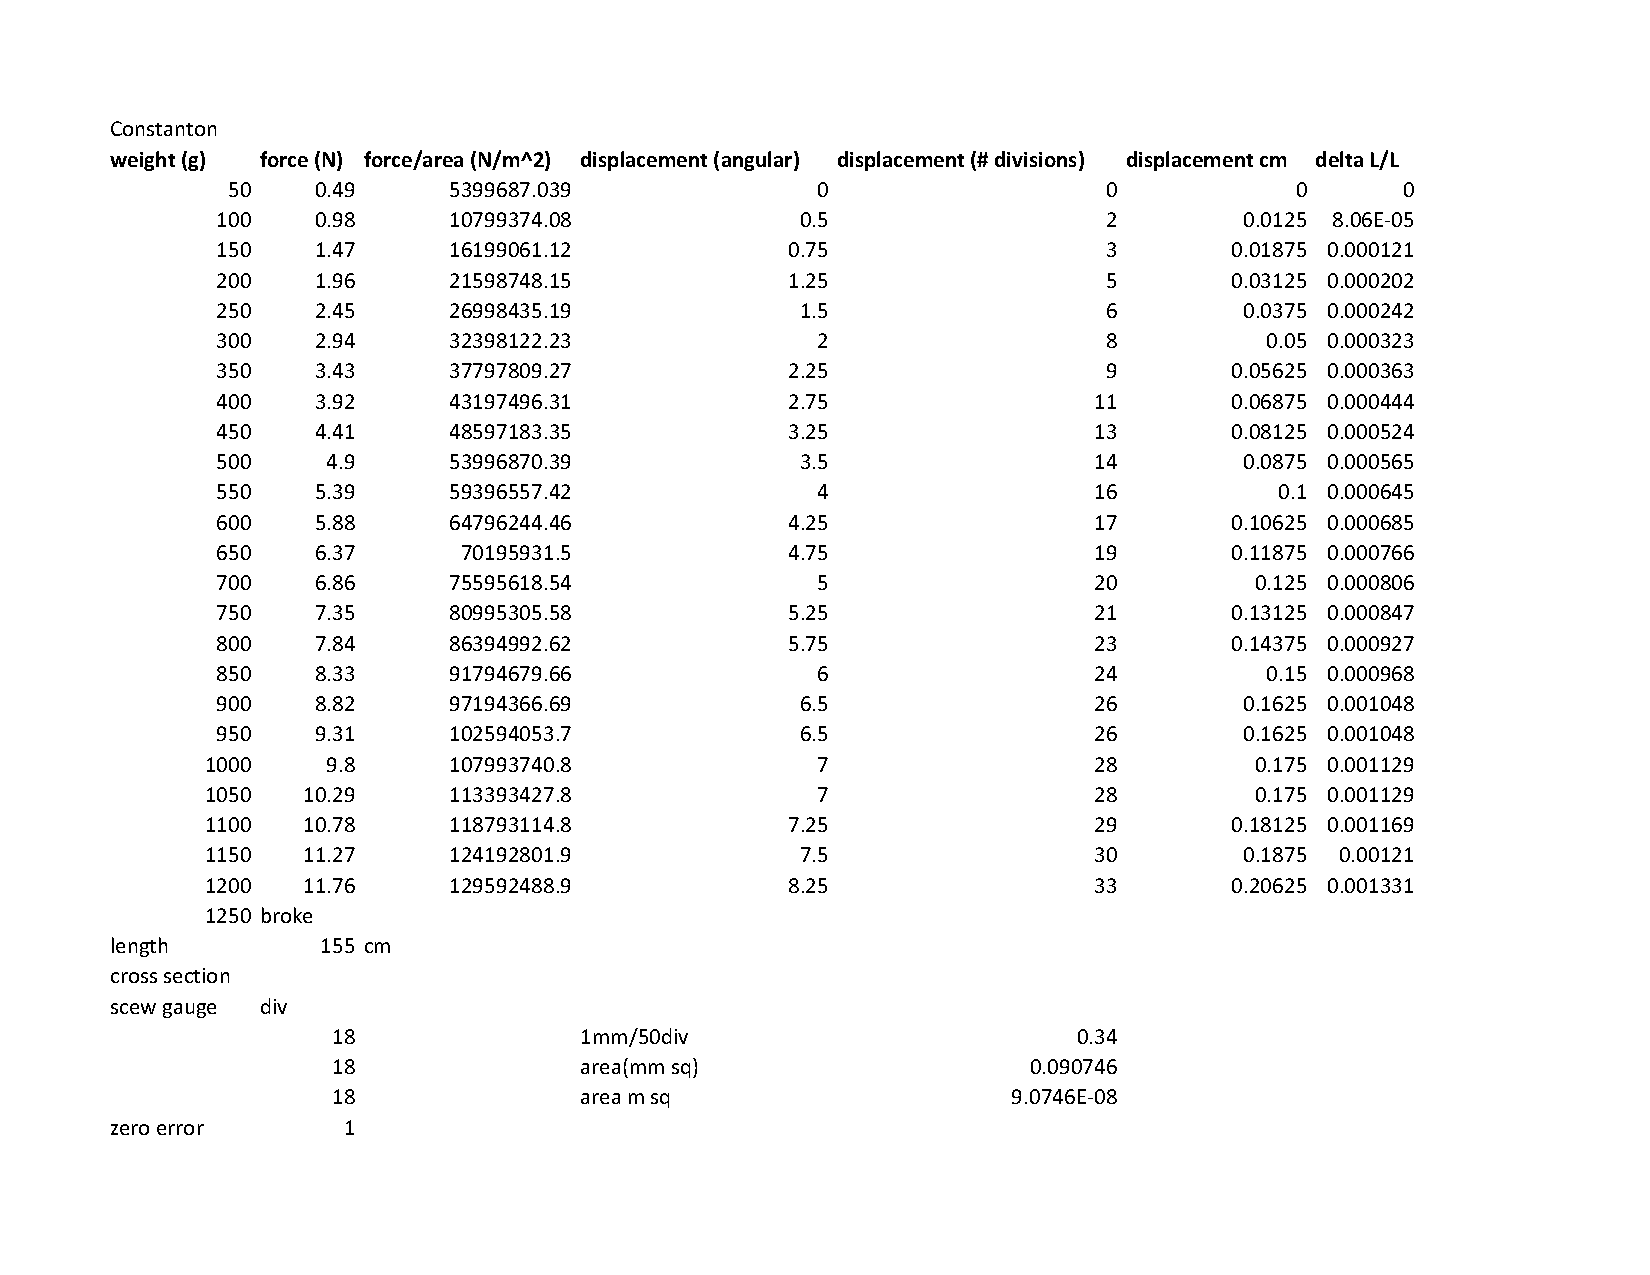
\includegraphics[width=16cm]{others/constanton-datafile}


\subsection{Copper}

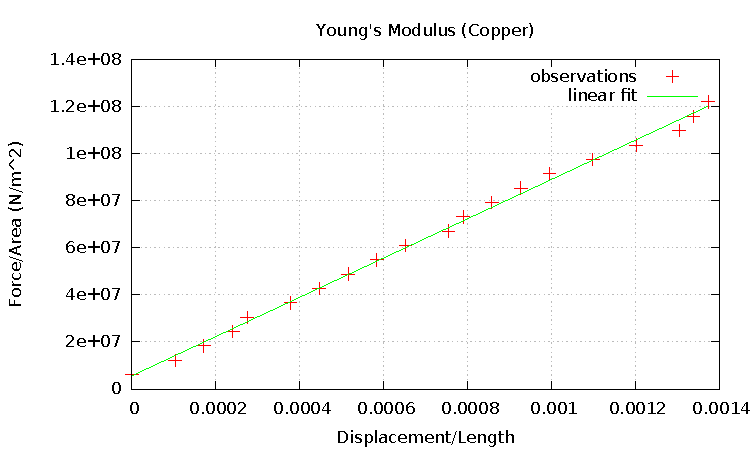
\includegraphics{exp5gnu/copper}

\lstinputlisting{exp5gnu/copperFit.tex}

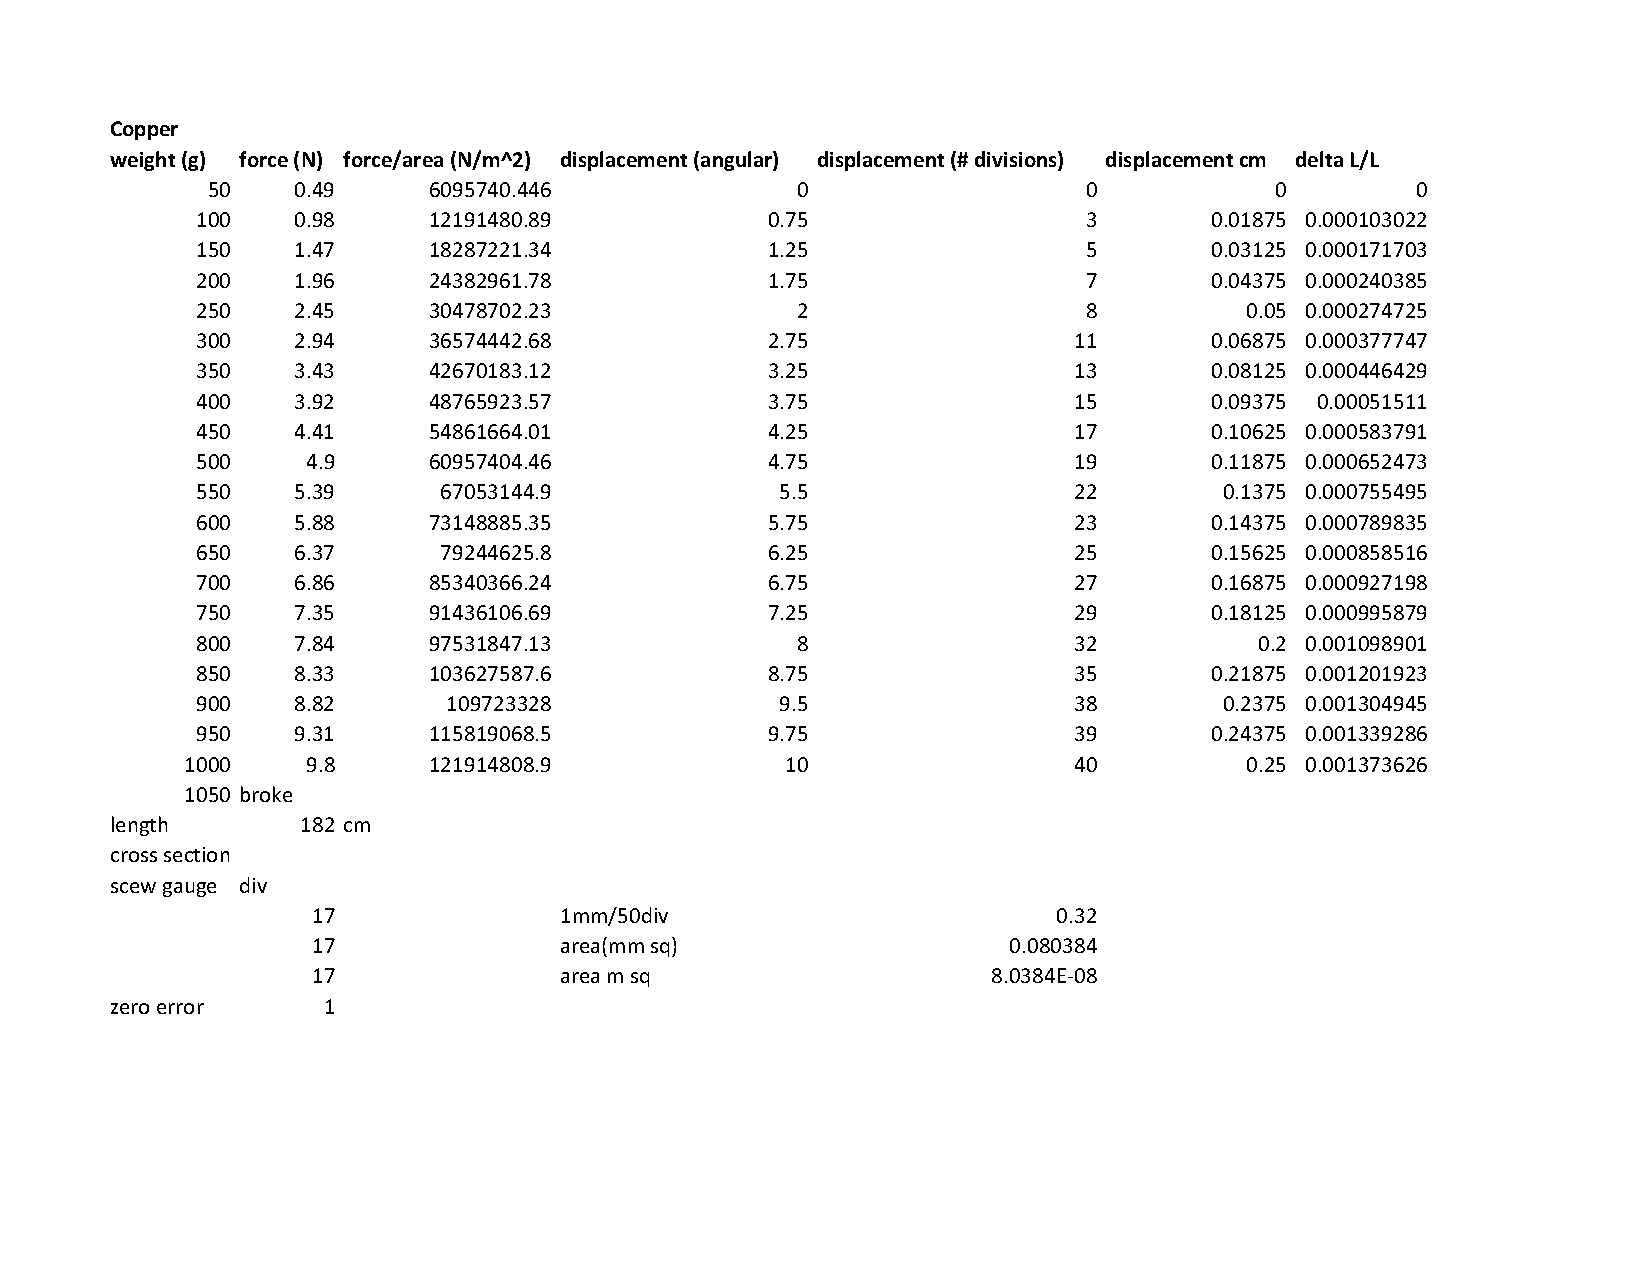
\includegraphics[width=16cm]{others/copper-datafile}


\subsection{Result}

The Young's modulus for Constantan was found to be $(9.500\pm0.178)\times10^{10}$
$N/m^{2}$ ($\sim2\%$ precision) and for Copper it was $(8.330\pm0.104)10^{10}$
$N/m^{2}$ ($\sim1\%$ precision). The breaking point of Constantan
was found to occur just beyond $(1.295\pm.0609)\times10^{8}$ $N/m^{2}$
while that of Copper was $(1.219\pm.0609)\times10^{8}$ $N/m^{2}$where
the error is caused by the smallest weight available ($50$ g).


\section{Critique}

The setup was not too shabby. The following improvements will reduce
performance time and increase accuracy
\begin{itemize}
\item Get thinner small weights (they can be wide)
\item Use a telescope to note $\Delta l$ instead of the angular measurement
apparatus
\end{itemize}
The angular dial has the following issues:
\begin{itemize}
\item the height of the dial has to be adjusted by trial
\item the range of the dial is restricted
\end{itemize}

\section{Acknowledgements}

I thank Prashansa Gupta and Vivek Sagar for their contribution in
the completion of this experiment. Further, as stated earlier, the
theory for this experiment has been primarily been adapted from \url{http://www.animations.physics.unsw.edu.au//jw/elasticity.htm}.
\end{document}
